\chapter{Results} 
  \section{Coherent cross section}
  For the coherent cross section, the raw yield of dimuon candidates was
    measured after applying the cuts described in Section~\ref{sec:DataSetEvSel}.
  \begin{figure}[!Hhtb]
    \centering
    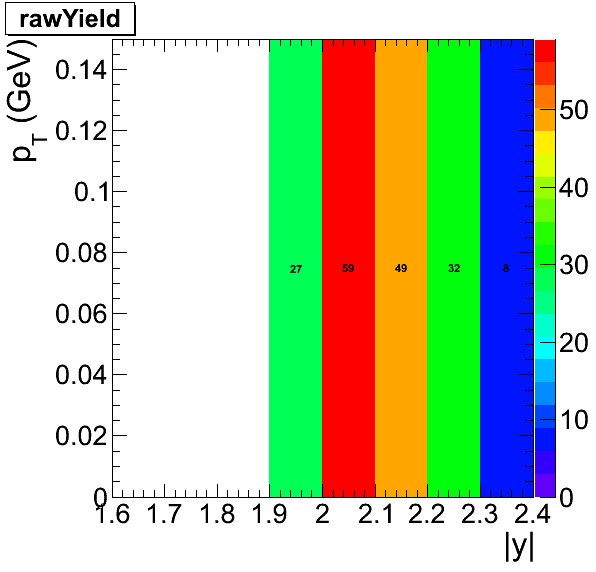
\includegraphics[width=0.6\textwidth]{rawYield}
    \caption{Raw yield for the Coherent cross section measurement.}
    \label{fig:rawYieldCo}
  \end{figure}

  The raw yields were divided by the total efficiency times acceptance factors
    to produce corrected yields.
  \begin{figure}[!Hhtb]
    \centering
    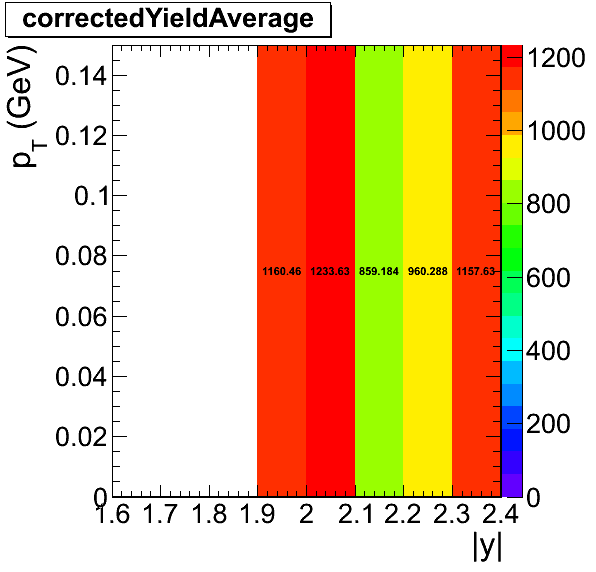
\includegraphics[width=0.6\textwidth]{correctedYieldAverage}
    \caption{Corrected yields for the coherent p$_{T}$ region.}
    \label{fig:corYieldCo}
  \end{figure}

  The corrected yields in the 2.0-2.1 and 2.1-2.2 $|y|$ rapidity bins were added 
    together to calculate the cross section. 
  These bins were selected to insure a total acceptance times efficiency 
    greater than 5\%.

  The contribution from coherent production was estimated from the template fit
    in Fig.~\ref{fig:ptTempFit}.
  The first three bins are used to estimate the contribution below 150 MeV.

  \section{Incoherent cross section}
  \section{Break up ratios}
    In Table~\ref{tab:r2} the ratio between raw yields for different break up 
      modes are shown.
    \begin{figure}[!Hhtb]
      \centering
      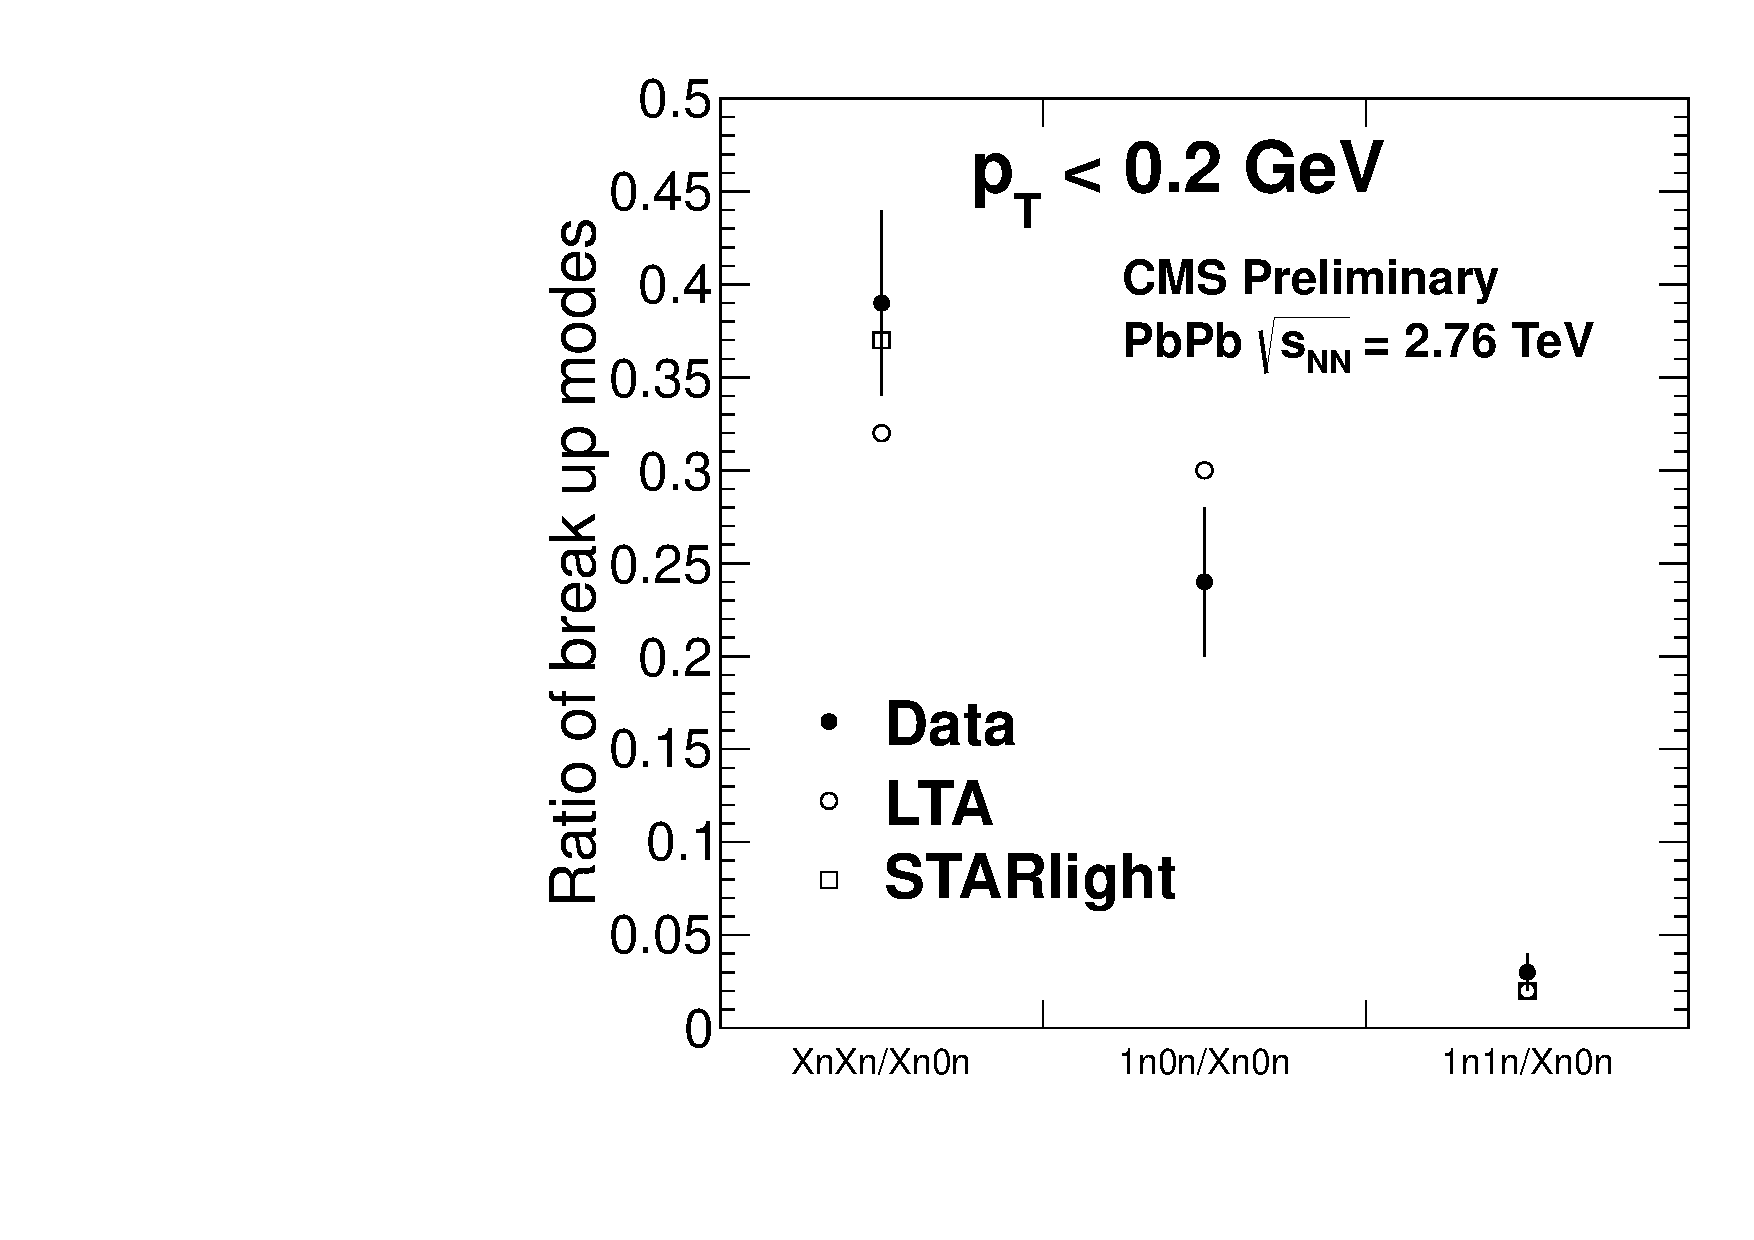
\includegraphics[width=.6\textwidth]{coherentBreakup}
      \caption{Ratio between J/$\psi$ yeilds XnXn and 1n0n break-up modes 
        compared the Xn0n break-up mode for J/$\psi$ with $p_{T}$ below 150 
        MeV.}
      \label{fig:coherentBreakUp}
    \end{figure}
   
    Fig.~\ref{fig:coherentBreakUp} and Fig.~\ref{fig:incoherentBreakUp} compare
      the raw break up ratios two STARlight and LTA predictions. 

    \begin{figure}[!Hhtb]
      \centering
      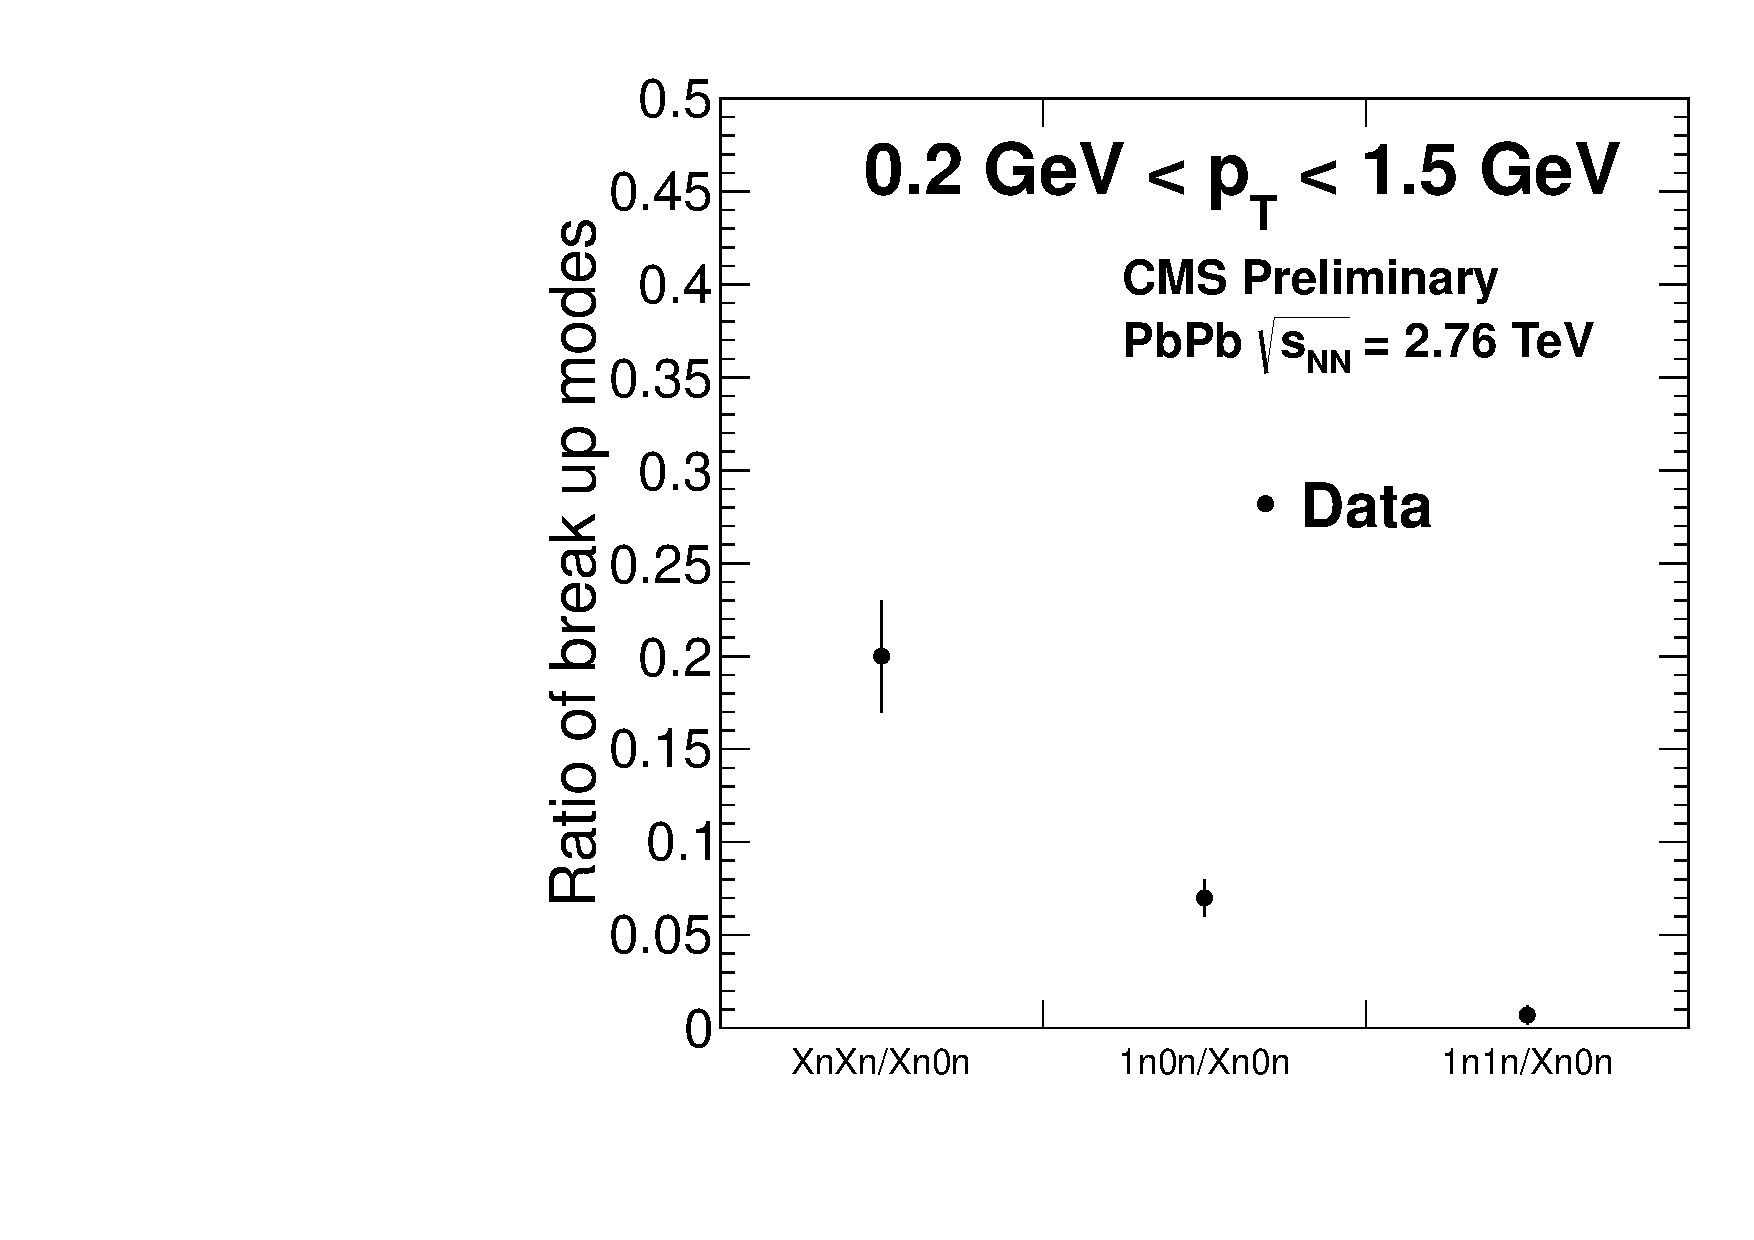
\includegraphics[width=.6\textwidth]{incoherentBreakup}
      \caption{Ratio between J/$\psi$ yeilds XnXn and 1n0n break-up modes 
        compared the Xn0n break-up mode for J/$\psi$ with 0.2 $< p_{T} <$ 
        1.5 GeV.}
      \label{fig:incoherentBreakUp}
    \end{figure}

    In Table~\ref{tab:r3} the ratio between break up modes are shown for 
      different theories and processes.

    \begin{table}[h]
      \begin{center}
        \caption{Number of  J/$\psi$ integrated over $p_{T}$ and $y$ with statistical uncertainty.}
        \label{tab:r3}
        \begin{tabular}{|c|c|c|c|c|}
          \hline
          & X$_{n}$X$_{n}$/X$_{n}$0$_{n}$ & 1$_{n}$0$_{n}$/X$_{n}$0$_{n}$ & 1$_{n}$1$_{n}$/X$_{n}$0$_{n}$  \\ 
          \hline
          STARlight coherent &  0.37&-&0.02\\
          \hline
          Zhalov coherent& 0.32&0.30&0.02\\
          \hline
          STARlight incoherent &  0.37&-&0.007$\pm$0.02 \\
          \hline
        \end{tabular}
      \end{center}
    \end{table}

  \section{diMuon-neutron correlations}
    The invariant mass distribution for different break-up modes is show for the coherent and incoherent J/$\psi$ on the Fig.~\ref{fig:r1} and Fig.~\ref{fig:r2} respectively. 
    \begin{figure*}[!Hhtb]
      \begin{center}
        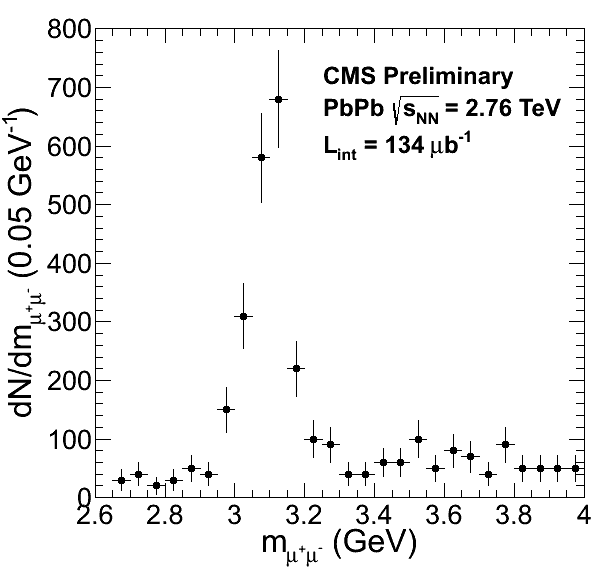
\includegraphics[angle=0,width=0.45\textwidth]{coherentJPsiMass.png}
        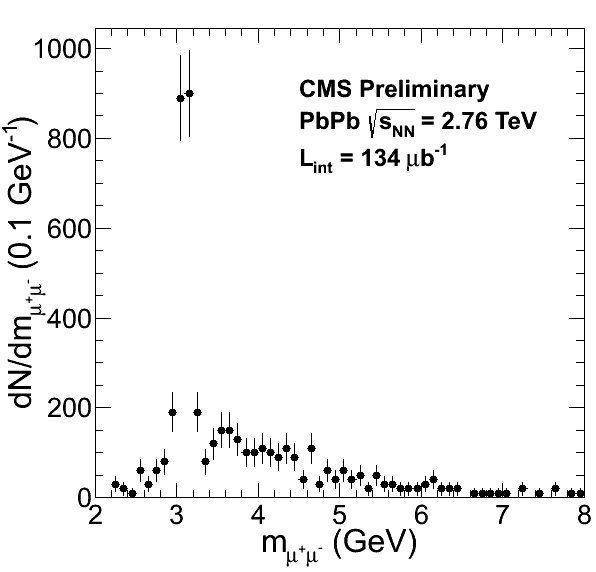
\includegraphics[angle=0,width=0.45\textwidth]{coherentMass.png}
        \caption{
          \label{fig:r1}  
          Invariant mass spectrum of the opposite signs di-muons originating from the coherent J/$\psi$ for $X_{n}0_{n}$ breakup mode for two invariant mass regions.  
        }
      \end{center}
    \end{figure*}
    
    \begin{figure*}[!Hhtb]
      \begin{center}
        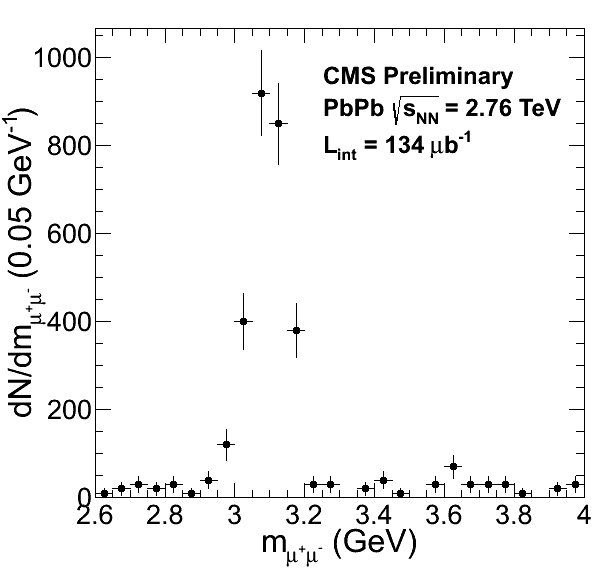
\includegraphics[angle=0,width=0.45\textwidth]{incoherentJPsiMassInCo.png}
        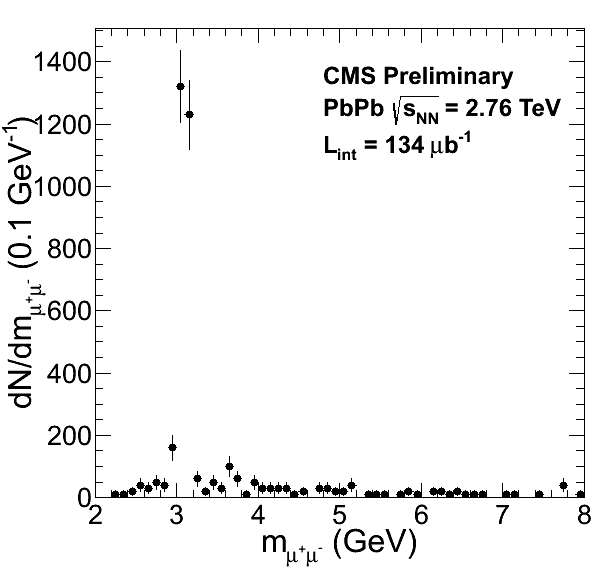
\includegraphics[angle=0,width=0.45\textwidth]{incoherentMassInCo.png}
        \caption{
          Invariant mass spectrum of the opposite signs di-muons originating
          from the incoherent J/$\psi$  for $X_{n}0_{n}$ breakup mode for two 
          invariant mass regions.   
        }
        \label{fig:r2}  
      \end{center}
    \end{figure*}
    
    The number of the coherent and incoherent J/$\psi$ for each break-up mode are
      given in the Tab.~\ref{tab:r1}. 
    The ratios between the modes X$_{n}$X$_{n}$, 1$_{n}$0$_{n}$, 1$_{n}$1$_{n}$ and
      the mode  X$_{n}$0$_{n}$ are given in the table Tab.~\ref{tab:r2}. 
    Some of the  ratios can be obtained from  {\sc starlight} and from the Zhalov 
      and thus are given in Tab.~\ref{tab:r3}.
    
    \begin{table}[h]
    \begin{center}
    \caption{Number of coherent J/$\psi$ integrated over $p_{T}$ and $y$ with statistical uncertainty.}
    \label{tab:r1}
    \begin{tabular}{|c|c|c|c|c|c|}
    \hline
                                   &  X$_{n}$0$_{n}$& X$_{n}$X$_{n}$ & 1$_{n}$0$_{n}$ & 1$_{n}$1$_{n}$  \\ 
    \hline
    coherent J/$\psi$ &  242$\pm$16&94$\pm$10&58$\pm$8&8$\pm$3\\
    \hline
     incoherent J/$\psi$ & 291$\pm$17&57$\pm$8&19$\pm$4&2$\pm$1  \\
    \hline
    \end{tabular}
    \end{center}
    
    \end{table}
    
    \begin{table}[h]
      \begin{center}
        \caption{Number of coherent J/$\psi$ integrated over $p_{T}$ and $y$ 
          with statistical uncertainty.}
        \label{tab:r2}
        \begin{tabular}{|c|c|c|c|c|}
          \hline
          & X$_{n}$X$_{n}$/X$_{n}$0$_{n}$ & 1$_{n}$0$_{n}$/X$_{n}$0$_{n}$ & 1$_{n}$1$_{n}$/X$_{n}$0$_{n}$  \\ 
          \hline
          coherent J/$\psi$ &  0.39$\pm$0.05&0.24$\pm$0.04&0.03$\pm$0.01\\
          \hline
          incoherent J/$\psi$ &  0.20$\pm$0.03&0.07$\pm$0.02&0.007$\pm$0.005 \\
          \hline
        \end{tabular}
      \end{center}
    \end{table}

   
    For statistical reason, further studies concentrate only on the break-up mode 
      X$_{n}$0$_{n}$. \\
    Figure~\ref{fig:r3} shows the transverse momentum distribution of the J/$\psi$ 
      (coherent and incoherent) in the case when J/$\psi$ and neutron have the same
      or opposite rapidity direction. 
    The ratio between the J/$\psi$ and neutron that have the opposite direction and
      the J/$\psi$ and neutron that have the same direction i shown on 
      Fig.~\ref{fig:r4}. 
    The red curve gives the pure theory calculations, the black one gives the theory 
      results that are injected to the detector simulation and thus taking into 
      account experimental bias. 
     
    \begin{figure*}[!Hhtb]
      \begin{center}
        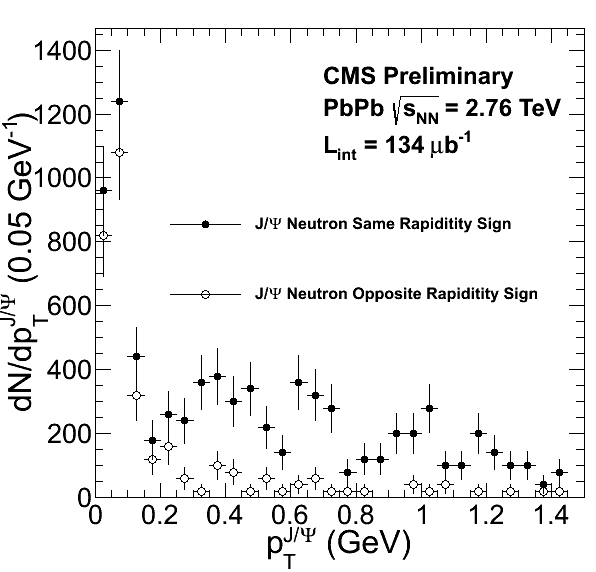
\includegraphics[angle=0,width=0.45\textwidth]{Pt.png}
            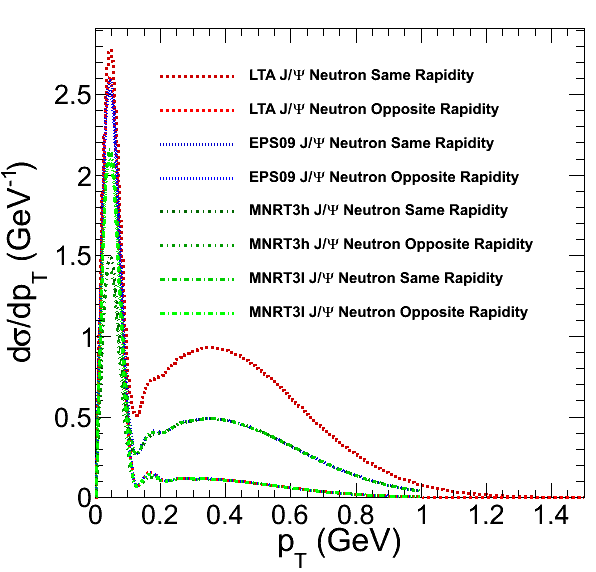
\includegraphics[angle=0,width=0.45\textwidth]{PtTheory.png}
                 \caption{
        \label{fig:r3}  
         Transverse momentum distribution of the J/$\psi$ when J/$\psi$ and neutron have the same or opposite rapidity direction from data (left) and from theory (right). 
            }
           \end{center}
    \end{figure*}
  
    \begin{figure*}[!Hhtb]
      \begin{center}
        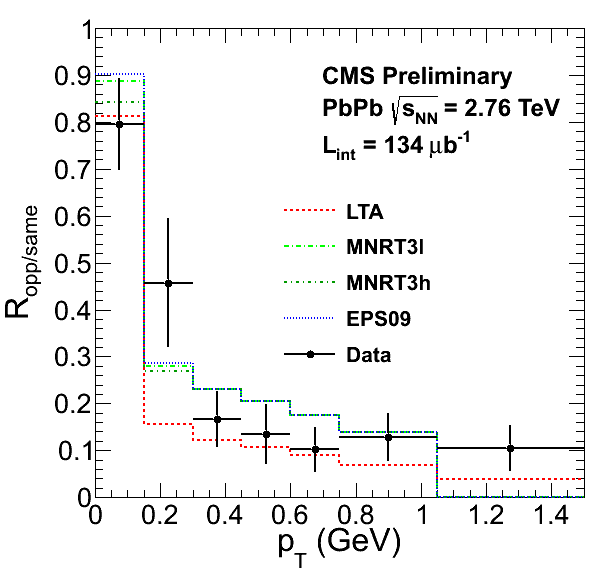
\includegraphics[angle=0,width=0.65\textwidth]{RoppSame.png}\\
                 \caption{
        \label{fig:r4}  
         Ratio between the transverse momentum distribution of the J/$\psi$ when  J/$\psi$ and neutron have the opposite direction and the transverse momentum distribution of the J/$\psi$ when  J/$\psi$ and neutron have the same direction. 
            }
           \end{center}
    \end{figure*}
    
    The rapidity distributions of the coherent and incoherent J/$\psi$ are shown in
      the Fig.~\ref{fig:r5}. 
    They are shown separately for the events firing the ZDC$^{+}$ and ZDC$^{-}$. 
    The same distributions are also obtained for the MC and shown in 
      Fig.~\ref{fig:r6}. 
    For the MC the particle gun generator with the input $p_{T}$ spectrum from 
      Zhalov's  calculation (LTA). 
    The rapidity symmetry for coherent J/$\psi$ and asymmetry for incoherent 
      J/$\psi$ are observed in data and MC. 
    These are quantified in the Tab.~\ref{tab:uref}. 
    
    \begin{figure*}[!Hhtb]
      \begin{center}
        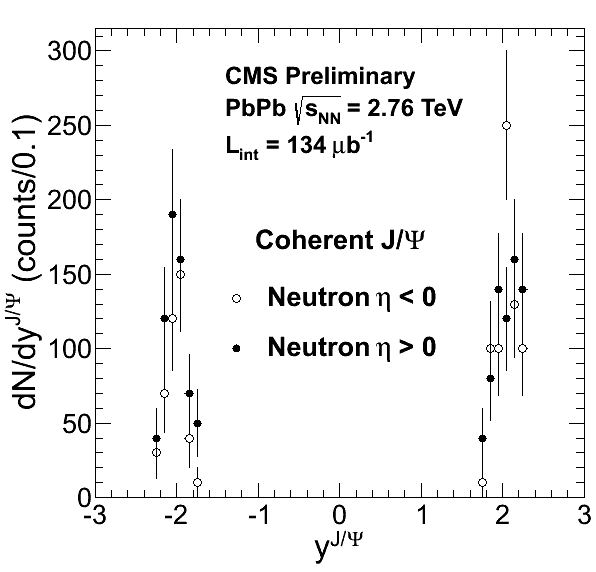
\includegraphics[angle=0,width=0.65\textwidth]{coherentRapidity1}\\
            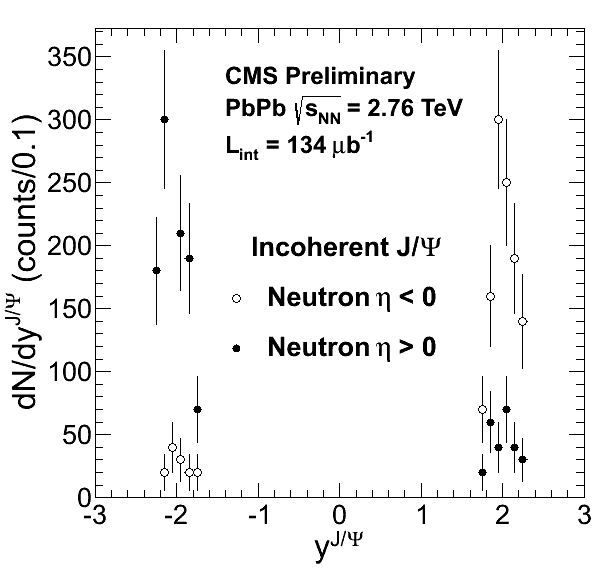
\includegraphics[angle=0,width=0.65\textwidth]{incoherentRapidity1}
             \caption{
        \label{fig:r5}  
        The rapidity distribution of the coherent (top) and incoherent (bottom) J/$\psi$ for the  ZDC$^{+}$ and ZDC$^{-}$. 
            }
           \end{center}
    \end{figure*}
    
    \begin{figure*}[!Hhtb]
      \begin{center}
        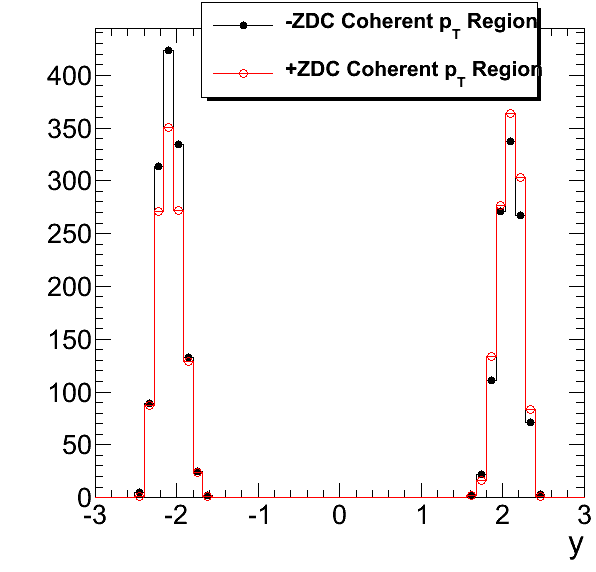
\includegraphics[angle=0,width=0.45\textwidth]{rapDistFromLTAGun.png}
            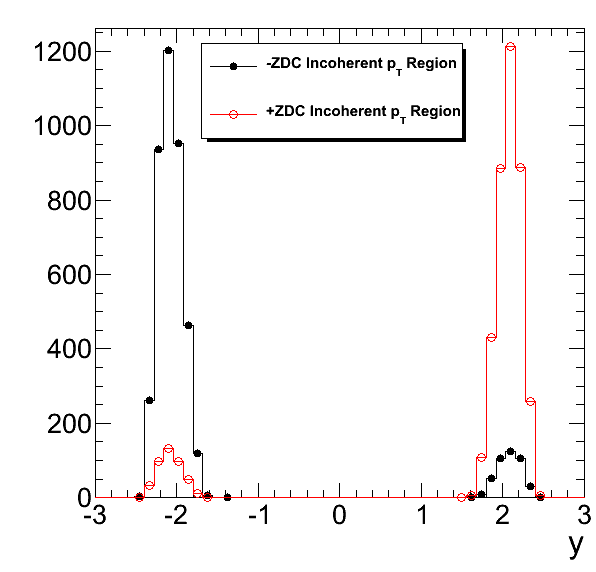
\includegraphics[angle=0,width=0.45\textwidth]{rapDistFromLTAGunInCo.png}
                 \caption{
        \label{fig:r6}  
          The rapidity distribution of the coherent (left) and incoherent (right) J/$\psi$ for the  ZDC$^{+}$ and ZDC$^{-}$ from MC (particle gun with customized $J/\psi p_{T}$ input distribution). 
            }
           \end{center}
    \end{figure*}
    
    Table~\ref{tab:uref} gives the number of coherent and incoherent J/$\psi$ 
      separately for the events that fired the ZDC$^{-}$ and ZDC$^{+}$. 
    We quote separately the J/$\psi$ that have the same or opposite rapidity 
      direction to the neutron direction. 
    The ratios, as described below are also given in the Tab.~\ref{tab:uref}: 
      $R_{ZDC^{-}}^{y^{+}/y^{-}}$ : ratio between the number of J/$\psi$ having 
        $y>0$ to the number of J/$\psi$ having $y<0$ from the events that fired 
        ZDC$^{-}$\\
      $R_{ZDC^{+}}^{y^{-}/y^{+}}$ : ratio between the number of J/$\psi$ having 
        $y<0$ to the number of J/$\psi$ having $y>0$ from the events that fired 
        ZDC$^{+}$\\
    
    \begin{table}[h]
    \begin{center}
    
    \caption{Final number of J/$\psi$ (for both ZDCs and for two negative and positive rapidity) and ratios with statistical uncertainty.}
    \label{tab:uref}
    \begin{tabular}{|c|c|c|c|c|c|c|}
    \hline
    & ZDC$^{-}$ $y<0$ & ZDC$^{-}$ $y>0$ & $R_{ZDC^{-}}^{y^{+}/y^{-}}$  & ZDC$^{+}$ $y<0$& ZDC$^{+}$ $y>0$& $R_{ZDC^{+}}^{y^{-}/y^{+}}$ \\ 
    \hline
    coherent J/$\psi$ & 63&68&1.08$\pm$0.19& 42&69 & 0.61$\pm$0.12 \\
    \hline
     incoherent J/$\psi$ &141 &26&0.184$\pm$0.039& 13&111& 0.117$\pm$0.034\\
    \hline
    \end{tabular}
    \end{center}
    
    \end{table}
    
    The combined ratio $R_{opp/same}^{c}$ is calculated as \\
      $$ R_{opp/same}^{c} = \frac{ZDC^{-} \mbox{and}~y>0 + ZDC^{+} 
      \mbox{and}~y<0}{ZDC^{-} \mbox{and}~y<0 + ZDC^{+} \mbox{and}~y>0} $$\\
    \begin{itemize}
      \item $ R_{opp/same}^{c}$ for coherent J/$\psi$= 0.83 $\pm$ 0.12.
      \item $ R_{opp/same}^{c}$ for incoherent J/$\psi$= 0.155 $\pm$ 0.021.
    \end{itemize}
    
    The correction factors (efficiency, reconstruction) are as following: 
    \begin{itemize}
      \item $\epsilon_{ZDC^{-}}$: efficiency of the ZDC$^{-}$ of 0.98
      \item $\epsilon_{ZDC^{+}}$: efficiency of the ZDC$^{+}$ of 0.94\ 
      \item $\epsilon_{\mu^{-}}$: efficiency $\times$ reconstruction of the muons 
        with rapidly $<$0: 1.0 
      \item $\epsilon_{\mu^{+}}$: efficiency $\times$ reconstruction of the muons 
        with rapidly $>$0: 1.014. 
    \end{itemize}
    
    The combined ratio  $R_{opp/same}^{ceff}$ corrected with the factors  above is 
      calculated as \\
      $$ R_{opp/same}^{ceff} = \frac{\epsilon_{ZDC^{-}} \epsilon_{\mu^{+}} ZDC^{-} 
        \mbox{and}~y>0 + \epsilon_{ZDC^{+}} \epsilon_{\mu^{-}} ZDC^{+} 
        \mbox{and}~y<0}{\epsilon_{ZDC^{-}} \epsilon_{\mu^{-}} ZDC^{-} 
        \mbox{and}~y<0 + \epsilon_{ZDC^{+}} \epsilon_{\mu^{+}} ZDC^{+} 
        \mbox{and}~y>0} $$
      $R_{opp/same}^{ceff}$ is 0.83$\pm$ 0.12.    \\
    
    \begin{itemize}
      \item $ R_{opp/same}^{ceff}$ for coherent J/$\psi$= 0.83 $\pm$ 0.12.
      \item $ R_{opp/same}^{ceff} $ for incoherent J/$\psi$= 0.154 $\pm$ 0.021.
    \end{itemize}
    
    If considering 3 significant figures for the representation of the result these
      values are: 
    \begin{itemize}
      \item $ R_{opp/same}^{c}$ for coherent J/$\psi$= 0.833 $\pm$ 0.124
      \item $ R_{opp/same}^{c}$ for incoherent J/$\psi$= 0.155 $\pm$ 0.021
      \item $ R_{opp/same}^{ceff}$ for coherent J/$\psi$= 0.828 $\pm$ 0.124
      \item $ R_{opp/same}^{ceff} $ for incoherent J/$\psi$= 0.154 $\pm$ 0.021
    \end{itemize}
    
    This shows that in this measurement the efficiencies factors are negligible. 
